\documentclass[12pt,a4paper]{article}
\usepackage{termpaper}
\usepackage[utf8]{inputenc}
\usepackage{graphicx}
\usepackage{listings}
\usepackage{xcolor}
\usepackage{cleveref}
\usepackage{filecontents}
\usepackage{minted}

\definecolor{lstcolor}{rgb}{0.95,0.95,0.95}

\lstdefinestyle{customc}{
  belowcaptionskip=1\baselineskip,
  breaklines=true,
  frame=L,
  xleftmargin=\parindent,
  language=C,
  showstringspaces=false,
  basicstyle=\footnotesize\ttfamily,
  keywordstyle=\bfseries\color{green!40!black},
  commentstyle=\itshape\color{purple!40!black},
  identifierstyle=\color{blue},
  stringstyle=\color{orange},
  tabsize=2
}
\lstset{escapechar=@,style=customc}

\newminted{c}{tabsize=2,fontsize=\footnotesize,bgcolor=lstcolor,linenos,breaklines}
\newmintinline{c}{bgcolor=lstcolor, fontsize=\footnotesize}
\newmintedfile{c}{tabsize=2,fontsize=\footnotesize,bgcolor=lstcolor,linenos,breaklines}

%opening
\title{Parallel breadth-first search}
\author{
 \authorname{Alexander Gallauner} \\
 \studentnumber{1026090} \\
 \curriculum{534} \\
 \email{alexander.gallauner@gmail.com}
}

\begin{document}
\maketitle
\begin{abstract}
To have a continuous progress of the performance of processors, it was necessary to concentrate on the development of multicore processors. With that development another problem was raising up. The programs or rather the algorithmic way of thinking have to be changed to get a speed up with multicore processors. It was the job of the developers to split up the work from one core to many cores and to coordinate the communication between these cores. In this report the focus is on algorithms for searching trees or graph data structures and how to parallelize them. To make it specific, we keep our mind on the breadth-first search, because it is easier to parallelize than the depth-first search. First there is a presentation of a sequential algorithm to solve that problem. After that a parallel realization of this sequential algorithm in pseudo code follows. We get an overview of the comparison between the sequential and parallel solution. After that there is a more concrete solution of the parallel algorithm with some implementation details. Additionally we show a history of changes or improvements of the parallel solution and how it influences the speed of the algorithm.
To get a feeling how good the solution is, there is an integration of our solution into a benchmark for supercomputers, the graph500 project. Graph500 establishes a large-scale benchmark for data-intensive supercomputer applications. There exists already a official solution of the benchmark, so we compare the performance of Jupiter, that is the name of the distributed system of the Vienna University of Technology, one time with the own implemented benchmark, but observing the rules of the graph500 project, and another time with the official solution of the graph500 project. With this results it is possible to compare Jupiter with some other supercomputers, listed in the graph500 ranking.
\end{abstract}

\clearpage

\section{The breadth-first search - BFS}
\label{sec:breadth-first search}

\subsection{Sequential BFS}
\label{sec:sequential-bfs}

\begin{listing}[h]
\begin{ccode}
/*
input: egde list as buffer
output: parent array
*/
BFS(edge_list, root){
	set_level(level, root);
	while level has nodes {
		for each Node n in level {
			for each Node m in neighbours(n){
				set_level(next_level, m);
				set_parent(parents, n, m); // sets the parent of m to n in parents
			}
		}
		level = next_level;
		clear(next_level);
	}
	return parents;
}
\end{ccode}
\caption{Sequential algorithm of the BFS.}
\label{lst:seq}
\end{listing}

The sequential BFS (breadth-first search) algorithm in Listing~\ref{lst:seq} is not difficult to understand. If we have a given tree or alternatively a graph data structure we start with a specific node. That is our root node. We can split the graph or tree into levels, each level is handled in one single iteration of the BFS. So we can say, we start with level 0 at the root node.
Then there starts the first round of the BFS. We take all nodes (root node for the first level) of the current level (that is level 0) and visit all neighbours of the nodes of the current level. All neighbours that have been visited are now the nodes of the next level (in this case that is level 1). The next step is to take all nodes of level 1 and visit all neighbours of these nodes. The BFS algorithm ends if the current level has no neighbours anymore or a specific search key is found. Output of the algorithm is a parent array, which contains parent information of each node. For better understanding the figure below shows a few iterations of the BFS algorithm.

\subsection{Parallel BFS}
\label{sec:parallel-bfs}

\begin{listing}[h]
\begin{ccode}
/*
input: for each processor - edge list as buffer of owned nodes, level information of owned nodes as array
output: parent array
*/
BFS_PAR(edge_list, level){
	while level has nodes {
		for each Node n in level {
			for each Node m in neighbours(n){
				set_level(next_level, m);
				set_parent(parents, n, m); // sets the parent of m to n in parents
			}
		}
		level = synchronize(next_level);
		clear(next_level);
	}
	return parents;
}
\end{ccode}
\caption{Parallel algorithm of the BFS.}
\label{lst:parallel}
\end{listing}

To make an algorithm parallel, the main problem is to split the work of the sequential algorithm into smaller pieces and assign that pieces of work to the existing processors of the system which are in use.  The first approach of splitting the BFS is to split the nodes of each level to the processors. Every processor of the system just visit the neighbours of the owned nodes. The problem with this approach is that the communication costs are pretty high, because it's necessary to split the work every round (level) of the BFS algorithm.\\
So the second and also chosen approach, illustrated in Listing~\ref{lst:parallel}, is to divide all the existing nodes and corresponding edges of the graph to the processors. With that approach the highest amount of communication is before the algorithm begins. After that the cores have to communicate in such a way, that they know which nodes are in the next level. That can happen in different ways, symbolized with \cinline/level = synchronize(next_level);/ but it is important that we have a parent array at the end of the algorithm. 

\section{Implementation of the BFS and some improvements}
\label{sec:implementations}

\subsection{Core of the parallel BFS solution}
\label{sec:core}
Here we will present our solution of the core of our parallel BFS algorithm in a more detailed pseudo code.\\
\begin{listing}[h]
\begin{ccode}
/*
input: every proc has adjacency buffer of owned nodes
output: parent array
*/
void BFS(buffer){
	char oneChildisVisited = 1;
	while (oneChildisVisited){
	oneChildisVisited = 0;
	for (i = 0; i < size(nodes_owned); i++){
		if (nodes_owned[i] is visited for the first time) {
			for (j = 0; j < size(neighbours); j++){
				if (neighbours[j] is not visited) {
					oneChildisVisited = 1;
					set_visited_bitmap(visited_bitmap, neighbours[j]); // sets the visited bitmap on position of neighbour[j] to 1
					save_parent(parent_array, nodes_owned[i]+1,neighbours[j]); // saves that nodes_owned[i]+1 is parent of neighbours[j] in parent array
				}
			}
		}	
	}
	allreduce(oneChildisVisited); // all procs get the information if there is a neighbour visited at all
	if (oneChildisVisited){
		allreduce(visited_bitmap, BITWISE_OR); // there has to be a reduction of all visited bitmaps to one
	}
	return parent_array;
}
\end{ccode}
\caption{Parallel BFS in more detail.}
\label{lst:detailedparallel}
\end{listing}
As Listing~\ref{lst:detailedparallel} shows, we need at first a flag \cinline/oneChildisVisited/. This flag keeps the information, if there is any new node visited. If not, all procs come to an end.\\
So if there is a new node in the current level, the procs have to iterate over the owned nodes and check if there is one of them in the current level and unvisited. If there is a new one in the current level, the proc iterates the neighbours of that node. For each neighbour there is a checking if it is set to 1 in the reduced visited bitmap and not visited in a level before. Is that the case the node is set to 1 in the visited bitmap and the owned node is saved as the parent of the neighbour node. After that the procs must reduce the \cinline/oneChildisVisited/ and \cinline/visited_bitmap/ information with the bitwise OR operation.

\subsection{Implementation details of the BFS}

In this section we will show some commands from the pseudo code in \ref{sec:core} and how to implement it in the programming language C with MPI. A good description of MPI is given by Rauber and R{\"u}nger \cite{rauber}. \\
Let us start with the first condition in the for-loop. 
\begin{ccode}
nodes_owned[i] is visited for the first time
\end{ccode}
This condition can be translated into
\begin{ccode}
position & level[((nodes_owned*my_rank+i) / BITS)] & ~visited[(i / BITS)]
\end{ccode}
where 
\begin{ccode}
position = (uint64_t) pow(2, (i % BITS));
\end{ccode}
We work with bitmaps of type \cinline/uint64_t/, so it is possible to save true or false (0 or 1) information of 64 nodes in one variable or field. To get the position of a node in a bitmap, we have to calculate two to the power of \(n\) where \(n\) is the number of the specific node modulo the count of possible bits, which is 64 in our case. For instance if our processor owns 256 nodes and we want to get the position of node number 90, our \(n\) is 26 and we calculate two to the power of 26. With that calculation we get the value, where the 26th bit is set to one.\\
The next step is to prove that the specific node is also set to one in the level array. The level array is a bitmap of all nodes of the graph and shows us which nodes were visited in the levels before. With \cinline/nodes_owned*my_rank+i/ we get the absolute position of the specific node, where \cinline/i/ is just the relative position. So if the absolute position is divided by the count of possible bits we get the correct field of the level array where the specific node is located. Let us show that with the example of node number 90 and with two processors where each processor has 256 nodes. There must be an level array with \(512/64 = 8\) fields and our node with number 90 must be at field number \((256*0+90) / 64 = 1\) where the fields begin with number 0 and the rank of the first processor is 0.\\
The visited array or bitmap gives us the information if a node is already visited or not. So if the bit of a specific node is set to one in the level array and the associated bit in the visited array is zero, we know through the bitwise AND operation \cinline/&/ that the node is visited for the first time. Otherwise if the bit in the visited array is one already, we know that the node was visited in a level or round before.\\
Assuming that the node was not visited before, we iterate over all neighbours of that node. With the condition \cinline/neighbours[j] is not visited/ translated to
\begin{ccode}
position & ~level[(buffer[j]/BITS)]
\end{ccode}
where
\begin{ccode}
position = (uint64_t) pow(2, (buffer[j] % BITS));
\end{ccode}
and \cinline/buffer[j]/ is one of the neighbours of the actual node, we check that this neighbour is visited in that level for the first time because of the synchronized level array, unless another node in the same level also visits that node, because he is also one of his neighbours. Here comes a race condition up, but for us it is enough that at the end the BFS tree represented through the parent array is correct.\\
If the condition evaluates to true we save the actual node as parent of the neighbour with
\begin{ccode}
parent_array[buffer[j]] = nodes_owned*my_rank+i+1;
\end{ccode}
where \cinline/parent_array/ is an array of type \cinline/uint64_t/ and is as big as the count of nodes of the whole graph. If we save a parent in the parent array, we always calculate \(+1\) to the number of the node to prevent, because the parent array is initialized with zero, that the node with number zero is the parent of all nodes which are not set during the BFS.\\
When all processors finished the actual level, the \cinline/oneChildisVisited/ flag is synchronized with the command \cinline/allreduce(oneChildisVisited)/, which can be translated to
\begin{ccode}
MPI_Allreduce(MPI_IN_PLACE, (void *) &oneChildisVisited, 1, MPI_CHAR, MPI_BOR, MPI_COMM_WORLD);
\end{ccode}
If this flag is true, the processors know that there must be a next level or round. So they also synchronize the level array with
\begin{ccode}
MPI_Allreduce(MPI_IN_PLACE, (void *)level, (pow(2,SCALE) / BITS), MPI_UNSIGNED_LONG, MPI_BOR, MPI_COMM_WORLD);
\end{ccode}
which was \cinline/allreduce(visited_bitmap, BITWISE_OR)/ in pseudo code. After the reduce operation the next level starts.

\subsection{History of our BFS algorithm}

The solution of the algorithm in section \ref{sec:implementations} was not our first approach to solve the BFS problem. Our first idea was to solve it with matrices where each element represents an edge between two nodes. The problem with this approach is that if we have a sparse matrix we have a high waste of memory. So it was our next idea to save only the edges that are existing and to leave out the rest. We decided to store all existing edges in a buffer and to work with an index array to find the edges of each node. So the next important question was if every processor has his own part of the buffer how should each processor share the information which nodes are in the current or next level of the BFS. So we came to the first version of the BFS implementation:

\subsubsection{First version - next level bitmap}
\label{sec:firstversion}

The first version of the algorithm is characterized by a next level bitmap, because every processor stores the information about new visited nodes in a next level bitmap which has a size of \(n\) bits where \(n\) is the count of nodes of the whole graph. So at every round the processors iterate over the owned nodes and check if the actual node in the iteration is in the current level and not visited. If that is the case the algorithm sets all bits of the neighbours of the current node in the next level bitmap to one. At the end of each round there must be a reduce scatter operation between the processors to ensure that every processor gets the level information of the next round.\\
The only problem with that approach is that it is difficult to create a parent array if you just synchronize a next level bitmap between the processors and it is not known who is the parent of the visited nodes. The disadvantage of that procedure is that the reduce scatter operation with a next level array of type \cinline/uint64_t/ takes time and the algorithm becomes inefficient with a higher count of processors.

\subsubsection{Second version - \cinline/uint64_t/ next level array}
\label{sec:secondversion}

In the second version of the algorithm we did not use a next level bitmap, instead we used a next level array of type \cinline/uint64_t/. At the position where we normally set the bit to one in the next level bitmap, we store the parent of the specific visited node. After the reduce scatter operation of the next level array, where every entry stores the parent of the node, every processor knows the parent of these nodes, which are already visited and which the processor owns. Unfortunately this approach is very inefficient because reducing the next level arrays in each round is really time-consuming and becomes more sophisticated with the increasing number of processors.

\subsubsection{Third and current version - visited bitmap}
\label{sec:thirdversion}

The basic idea of this approach is that that we do not have a next level bitmap or array, we always keep a bitmap of all visited nodes in all levels synchronized. All processors know which node is already visited and which not and the parent of each node can be correctly stored at each processor. Before the algorithm ends the parent arrays of each processor get combined to one parent array with an allreduce operation. Section \ref{sec:implementations} gives detailed information about this approach.\\
If you want to study the algorithm and the history of that algorithm in a more detailed way, you can check the appendix of this paper. There is the source code at \ref{sec:sourcecode}  of every version in fully length.

\section{Testing the algorithm on Jupiter}
\label{sec:testing}

For better understanding how changes in the algorithm influence the speed of the algorithm we compare the results of the different versions on Jupiter. In the following figures we work with a graph of scale 25 and an edgefactor of 4. That means that we have \(2^{25}\) nodes and \(2^{27}\) edges. The edges were generated by a kronecker graph generator, researched by Leskovec, Chakrabarti, Kleinberg, Faloutsos and Ghahramani  \cite{kronecker}.

\subsection{Testing the first version}

Let us start with the first version from section \ref{sec:firstversion}.

\begin{figure}[!ht]
   \centering
   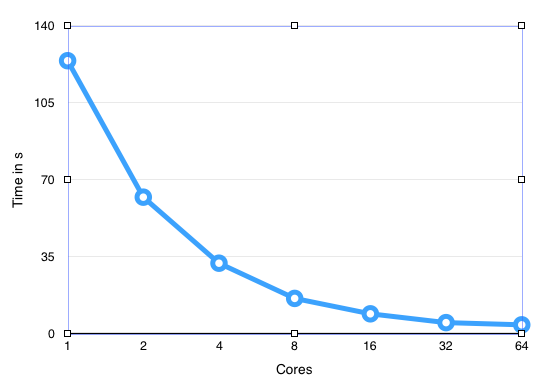
\includegraphics[width=0.75\textwidth]{next_level}
   \caption{Results of the next level bitmap approach.}
   \label{fig:nextbitmap}
\end{figure}

Figure~\ref{fig:nextbitmap} shows the results of the first version of our algorithm. There is a quite good speedup with a higher number of cores, but the problem, like mentioned in Section~\ref{sec:firstversion}, is that we do not have a parent array at the end of this algorithm and it is hard to extend this approach to get one.

\subsection{Testing the second version}

\subsection{Testing the third version}

\section{The graph500 project and my own realisation}
\label{sec:graph500}

In this section will be an implementation of the parallel BFS in MPI. The programming language is C, MPI is used to ensure the parallel solution. For more information about MPI read Rauber 2013 (reference not working :( , in progress)\\
Because it would be too costly to type in the node data for a scale of \(2^{32}\) or higher, the first part of the program is to generate nodes. For the data generation we used a Kronecker generator. Later in this paper there will be a section of this Kronecker generator, which creates natural graphs. In an own program the kronecker generator generates an edge list, containing start vertices and end vertices. These edge list will be written into a file, so the graph don't have to be generated each time for new. For generation the following void function will be used:

\begin{lstlisting}
generate_graph(SCALE, EDGEFACTOR, initiator, startVertex, endVertex);
\end{lstlisting}

In this line the Kronecker generator fills the \lstinline{startVertex[i]} and \lstinline{endVertex[i]} arrays with random numbers of nodes. Each pair of \lstinline{startVertex[i]} and \lstinline{endVertex[i]}, for \( 0 < i < N, N = count of nodes \) is representing an edge of the graph. The \lstinline{SCALE} parameter gives the generator the size of the graph and the \lstinline{EDGEFACTOR} the ratio of the count of the edges to the count of the nodes. The \lstinline{initiator} is a 2x2 map, filled with probabilities, which influences the functioning of the Kronecker generator. So after the generation our root proc reads the graph data from the file and brings the information in a more computeable form.

\begin{lstlisting}
create_node_edge_lists(nodes, edges, startVertex, endVertex, node_edge_list, count_edges_per_node);
\end{lstlisting}
Firstly the arrays of vertexes are converted to an array of nodes, where each entry of the array points to a list of nodes, which are neighbours of this specific entry.
\begin{lstlisting}
buffer = lists_to_buffer(&buffer_size, node_edge_list, count_edges_per_node, 0, nodes-1);
\end{lstlisting}
Secondly that array of nodes, where each entry points to a list, is transformed to a buffer, where the neighbours of the node 1 are at the beginning of the buffer, then the neighbours of the node 2 follow the neighbours of node 1, and so on.
The next step is to calculate the amount of edges each proc of the system is receiving, so that the procs can allocate the necessary memory for their part of the buffer and scattering it from the root proc to all procs.  So far we just handled functions, which were only processed by the root proc, but from now the functions in the future get called by the root AND all other procs. \\
After that calling the function
\begin{lstlisting}
MPI_Scatterv((void *) buffer, buffer_send_counts, buffer_displs, MPI_UINT64_T, (void *) buffer_recvbuf, buffer_recv_size, MPI_UINT64_T, 0, MPI_COMM_WORLD);
\end{lstlisting}
the \lstinline{buffer} is scattered to all procs, which have already allocated the necessary space. \lstinline{buffer_send_counts} gives the information, how many units each proc gets. \lstinline{buffer_displs} is a vector, whichs shows the starting index of the buffer for each proc, so the right part of the entire buffer is scattered for each proc. \lstinline{buffer_recvbuf} ensures that every proc has a buffer to store the received information.\\
As we already above-mentioned at the explanation of our approach of the parallel BFS there has to be a thinking in levels and there has to be a communcation, which procs must work at the next round/level. For instance at the beginning the root node is in the first level (level 0). So just the proc, which is responsible for the root node, is working in the first round. The next step is that the neighbours of the root node have their turn. All procs, which own one node of the second level, have to work in the next level. With
\begin{lstlisting}
MPI_Scatter((void *)level,nodes / BITS / procs,MPI_UNSIGNED_LONG, (void *)level_recvbuf, nodes / BITS / procs, MPI_UNSIGNED_LONG, 0, MPI_COMM_WORLD);
\end{lstlisting}
the nodes of the first round get scattered. \lstinline{level} is a bitmap of type \lstinline{unsigned long} with the nodes of the current round set to 1. \lstinline{nodes / BITS / procs} says how many units of type \lstinline{unsigned long} every proc (including the root node) is receiving. \\
At the next instruction the procs (also the root proc) comes to the most relevant function of the algorithm.
\begin{lstlisting}
bfs(level_recvbuf, buffer_recvbuf, buffer_recv_size, count_edges_per_node_recvbuf, (nodes / procs), procs);
\end{lstlisting}
Here is the beginning of the basic algorithm of our parallel BFS algorithm. All steps so far were a preparation. The edge list was transformed into a better computeable form and the root node had to scatter some important data to the other procs of the system.

\section{Ranking of Jupiter}
\label{sec:ranking}

\section{Why no parallel realisation of depth-first search?}
\label{sec:depth-first search}

\section{Summary}
\label{sec:summary}

\clearpage

\nocite{*}
\bibliographystyle{abbrv}
\bibliography{bachelor}

\appendix
\section{Source Code}
\label{sec:sourcecode}
\cfile{../Source/bfs_par.c}
\clearpage
\lstinputlisting[caption={Kronecker Generator},label=kronecker_generator]{../Source/kronecker_generator.c}
\clearpage
\lstinputlisting[caption={project.h},label=project]{../Source/project.h}

\clearpage


\end{document}